% Created 2023-08-25 vie 23:10
% Intended LaTeX compiler: pdflatex
\documentclass[11pt]{article}
\usepackage[utf8]{inputenc}
\usepackage[T1]{fontenc}
\usepackage{graphicx}
\usepackage{grffile}
\usepackage{longtable}
\usepackage{wrapfig}
\usepackage{rotating}
\usepackage[normalem]{ulem}
\usepackage{amsmath}
\usepackage{textcomp}
\usepackage{amssymb}
\usepackage{capt-of}
\usepackage{hyperref}
\usepackage{../modern}
\bibliography{fuentes.bib}
\raggedbottom
\setcounter{secnumdepth}{2}
\author{Luis Eduardo Galidno Amaya}
\date{25 de Agosto del 2023}
\title{Conocer que es la Seguridad en \\
redes de cómputo y los diferentes elementos que la integran}
\hypersetup{
 pdfauthor={Luis Eduardo Galidno Amaya},
 pdftitle={Conocer que es la Seguridad en \\
redes de cómputo y los diferentes elementos que la integran},
 pdfkeywords={},
 pdfsubject={},
 pdfcreator={Emacs 27.1 (Org mode 9.3)}, 
 pdflang={Spanish}}
\begin{document}

\modentitlepage{../images/escudo-uabc-2022-1-tinta-pos.png}
\datasection{Individual}


\section{Definiciones seguridad en red}
\label{sec:org6c4bf58}
\subsection{Definición 1}
\label{sec:orgaa7166d}
\autocite{barney_lutkevich_2022}  La seguridad de red abarca todos los pasos tomados para proteger la integridad de una red de computadoras y los datos dentro de ella. La seguridad de red es importante porque mantiene los datos sensibles a salvo de los ciberataques y asegura que la red sea utilizable y confiable. Las estrategias exitosas de seguridad de red emplean múltiples soluciones de seguridad para proteger a los usuarios y las organizaciones del malware y los ciberataques, como el ataque distribuido de denegación de servicio (DDoS).

\subsection{Definición 2}
\label{sec:orgd6f4f01}
\autocite{Prabhu_24_2021} La seguridad de red se define como el proceso de crear un enfoque defensivo estratégico que asegura los datos de una empresa y sus recursos en toda su red. Protege a la organización contra cualquier forma de amenaza potencial o acceso no autorizado. Independientemente del tamaño de la organización, la industria o la infraestructura, las soluciones de seguridad de red la protegen contra la amenaza en constante evolución de los ciberataques.

\subsection{Definición 3}
\label{sec:org4b47779}
\autocite{Naz_2023} La definición aceptada a nivel global es que la seguridad de red es un sistema que protege múltiples aspectos como la tecnología, los dispositivos y los procesos. Protege los datos confidenciales tanto de las tecnologías de hardware como de software. Las empresas, independientemente de su tamaño, están utilizando la seguridad de red.

\section{Mapa mental}
\label{sec:org1113ec5}
\begin{figure}[htbp]
\centering
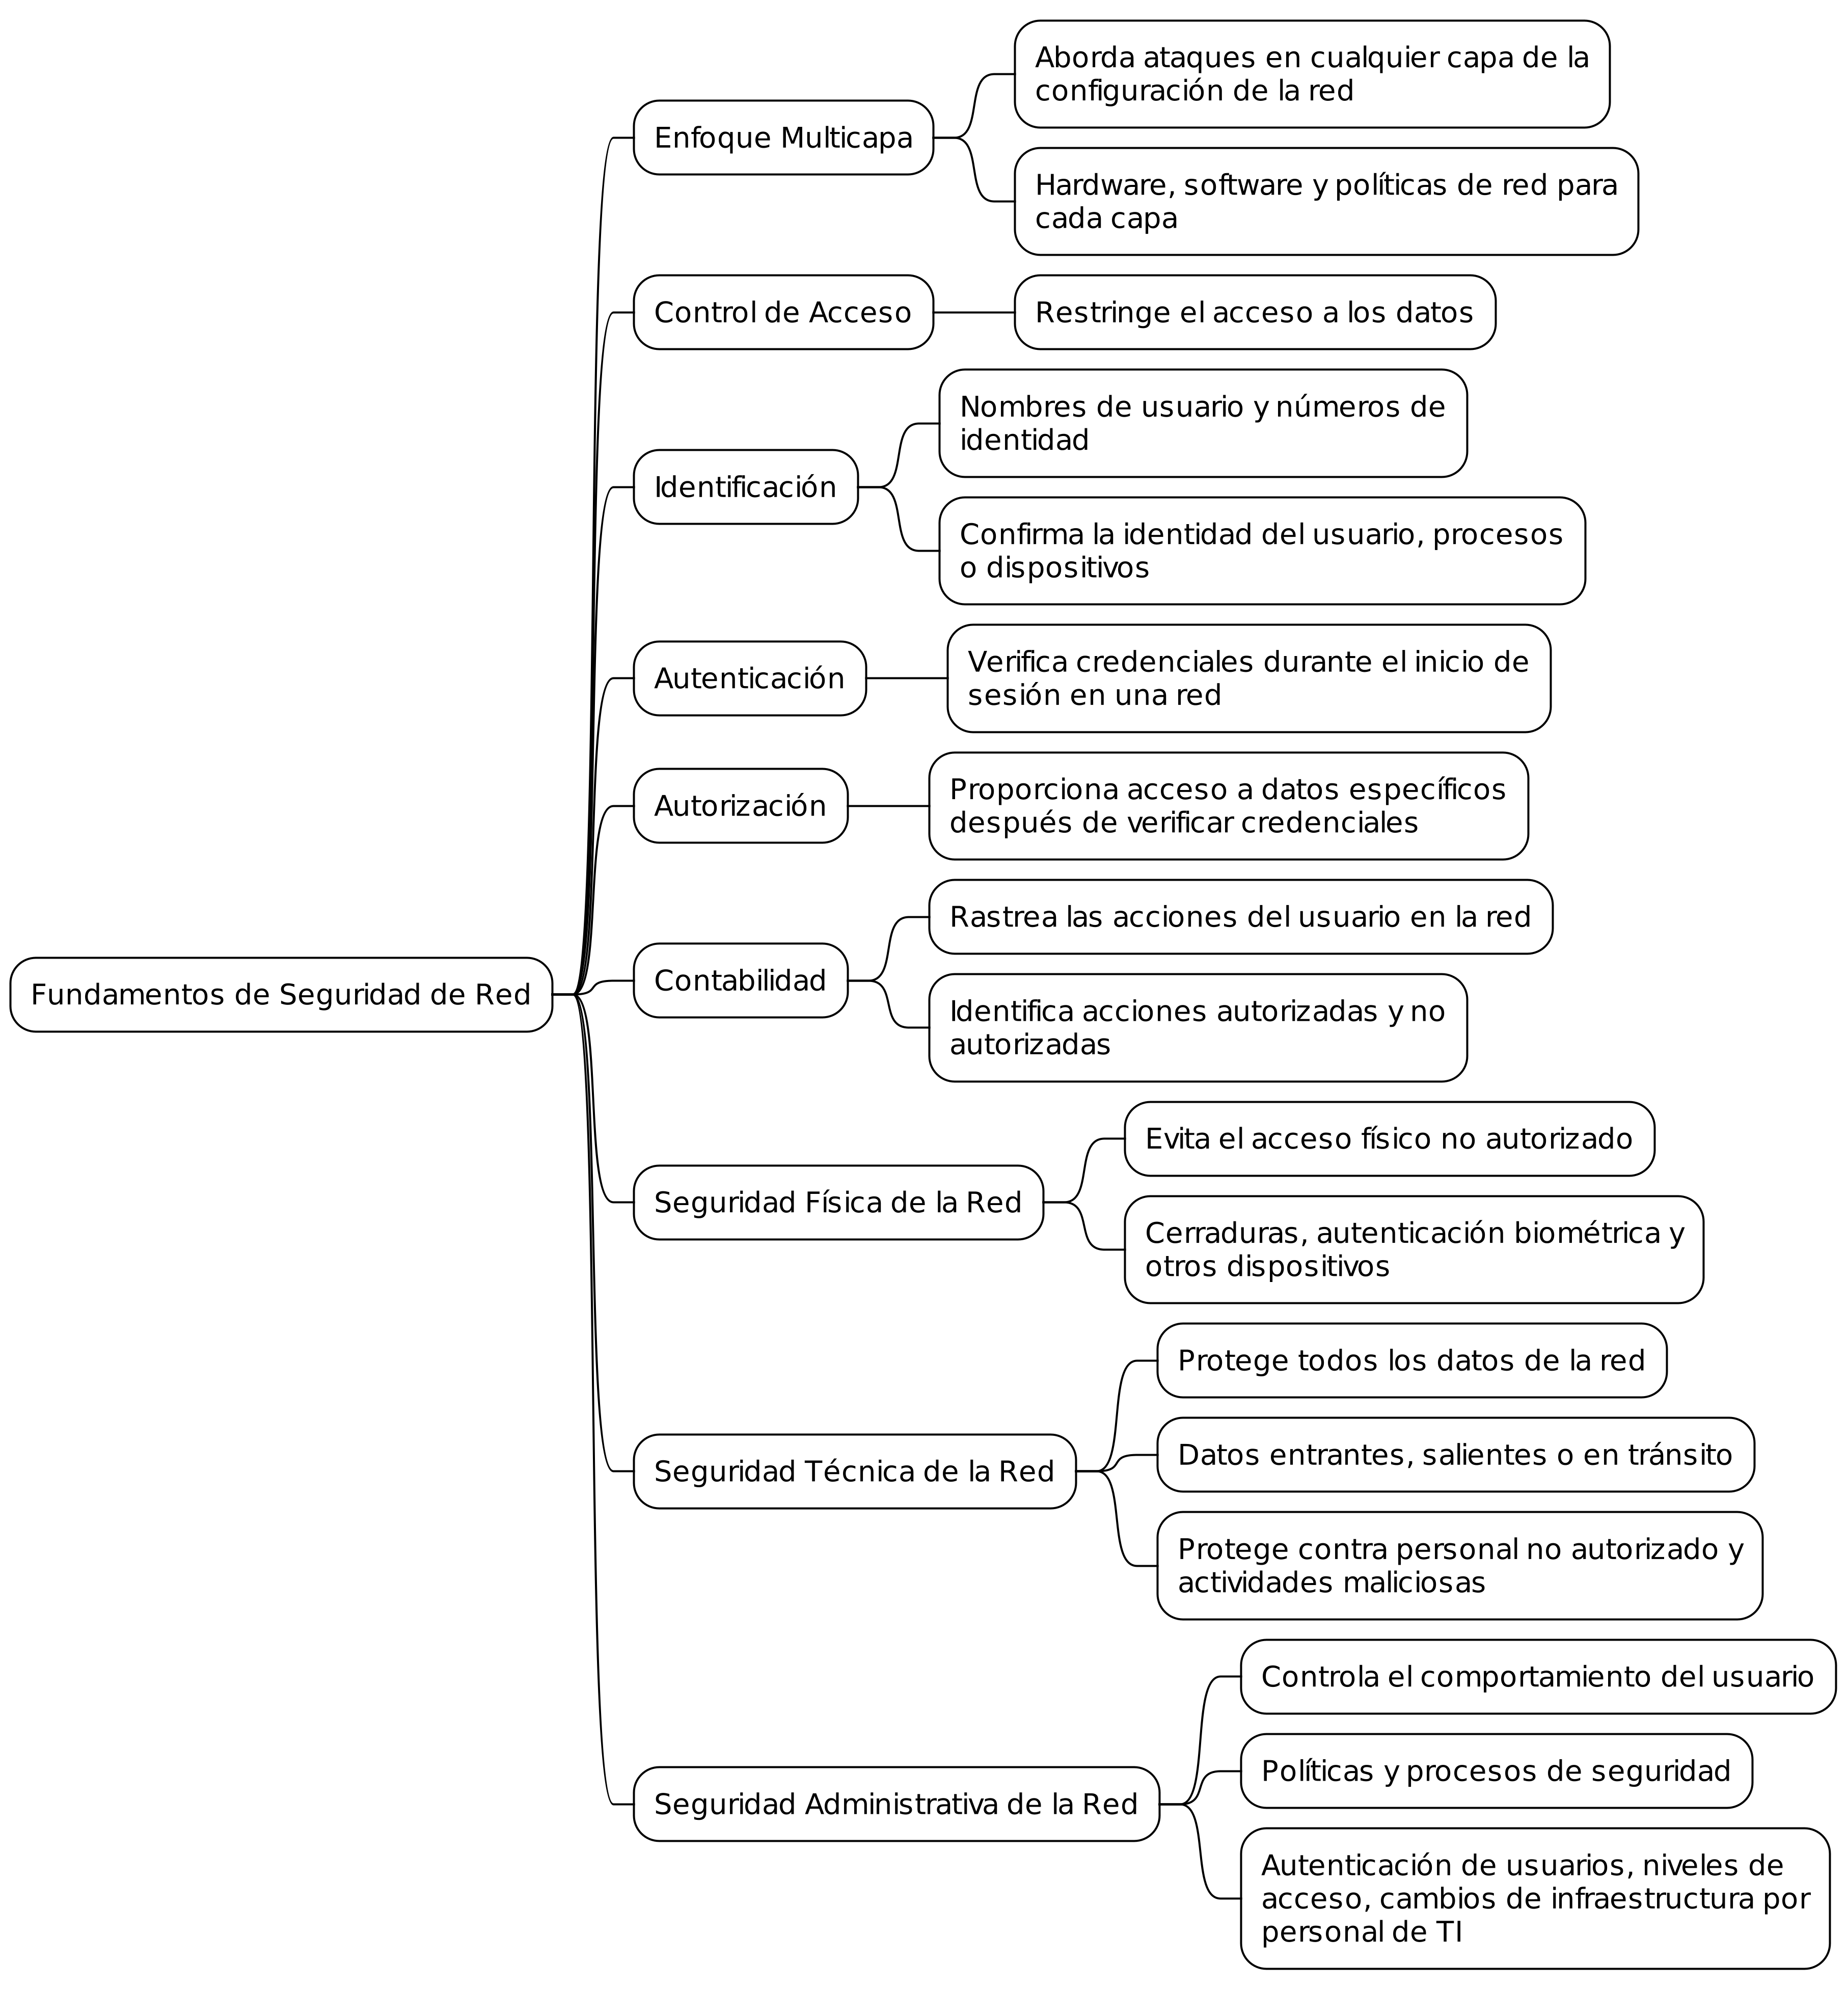
\includegraphics[width=.9\linewidth]{./images/diagram.png}
\caption{Fuentes \cite{Naz_2023}}
\end{figure}


\section{Referencias}
\label{sec:org42a7736}
\printbibliography[heading=none]
\end{document}
